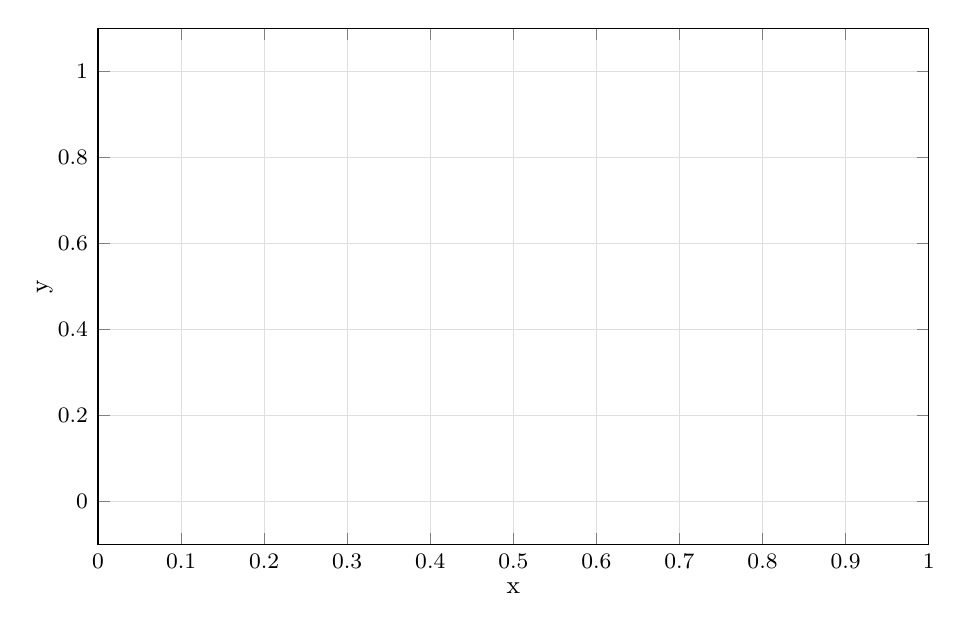
\begin{tikzpicture}
	\begin{axis}[
		width=0.87\linewidth, % Approximately full line width
		height=0.87\linewidth/1.61, % Golden ratio
		scale only axis,
		%title={My fancy plot of {$filename}},
		%title style={at={(0.5,0.95)}},
		xlabel={$$x$$},
		ylabel={$$y$$},
		legend entries={},
		%xtick distance=1,
		%ytick distance=1,
		grid=major,
		grid style={gray!25},
		%ymin=0,
		%ymax=1,
		enlarge x limits = false,
		%enlarge y limits = 0.05, % To reduce y-axis margins
		title style={font=\small},
		legend style={
			font=\footnotesize,
			%at={(0.5,0.5)}, % To reposition legend
			%legend pos = south west, % To reposition legend
			cells={anchor=west},
		},
		label style={font=\small},
		tick label style={font=\footnotesize},
		xlabel shift={-2},
		ylabel shift={-5},
		line width = 0.6pt,
		%clip mode=individual, % Force the marks to be behind lines
	]
		%\addplot[blue] table[x=x, y=y, col sep=comma] {$filename};
		%\addplot[red] table[x=x, y=y2, col sep=comma] {$filename};
	\end{axis}
\end{tikzpicture}%